\newpage
\section{Descrizione architettura}
\subsection{Metodo e formalismo di specifica}
Le scelte progettuali di MaaS sono state frtemente influenzate dallo stack tecnologico usato. \\
MaaS è basato su Node.js, e conseguentemente è scritto in JavaScript; questo linguaggio lascia molta libertà al programmatore nella scelta della tecnica da utilizzare per implemetare pattern come l'incapsulamento e l'ereditarietà. Al contrario di altri linguaggi orientati agli oggetti, come C++ o Java, non è presente un costrutto esplicito per definire classi, né un controllo statico dei tipi utilizzati. Per questo il team ha scelto, soprattutto per la codifica dell'editor visuale, di utilizzare il linguaggio TypeScript, che aggiunge, come già detto, la possibilità di definire classi ed interfacce. \\
La progettazione è stata influenzata pesantemente anche dal framework back end scelto: ExpressJS. Questo framework è basato su Node.js e permette di estenderlo attraverso moduli specifici secondo i bisogni dell'applicazione. Il concetto centrale è quello delle funzioni middleware, ovvero funzioni che hanno accesso all'oggetto richiesto dal client (req), all'oggetto di risposta del server (res) e alla successiva funzione middleware nel ciclo di risposta dell'applicazione (next()). Tipicamente le funzioni middleware possono eseguire le seguenti operazioni:
\begin{itemize}
\item Eseguire codice generico.
\item Cambiare gli oggetti req e res.
\item Terminare il ciclo di risposta dell'applicazione.
\item Richiamare il successivo middleware nello stack (next()).
\end{itemize}
Per soddisfare le richieste del proponente, ExpressJS verrà integrato con moduli per gestire il login (con base su MongoDB) e per inviare email agli utenti. \\
La progettazione della parte back end ha seguito un approccio top-down: inizialmente sono stati definiti i componenti principali del sistema, le relazioni tra essi ed infine l'interfaccia REST (\textbf{RE}presentational \textbf{S}tate \textbf{T}ransfer) da esporre al client. \\
I diagrammi delle classi permettono di mostrare l'architettura generale del sistema, ma in un mondo orientato alle funzioni non sono sufficienti per descrivere l'intero sistema. Per questo, vengono mostrati anche diagrammi di sequenza e attività, che permettono di definire le interazioni tra le componenti, senza preoccuparsi della loro classificazione. In questo modo è possibile esprimere alcuni meccanismi tipici di un'applicazione REST like, come il modo in cui agiscono i middleware. 
%todo frontend!!!!!!!!!
I diagrammi di deployment, dei package, delle classi, di sequenza e di attività presentati utilizzano la specifica UML (\textbf{U}nified \textbf{M}odeling \textbf{L}anguage) 2.0.
\subsection{Architettura generale}
L'architettura del progetto si divide in una componente Client, rappresentata dal browser degli utenti che interagiscono con il front end, e in una componente WebServer, nella quale risiede il back end. Il database MongoDB verrà posto su un altro server, possibilmente quello su cui risiede il front end. \\
\begin{figure}[h]
\centering
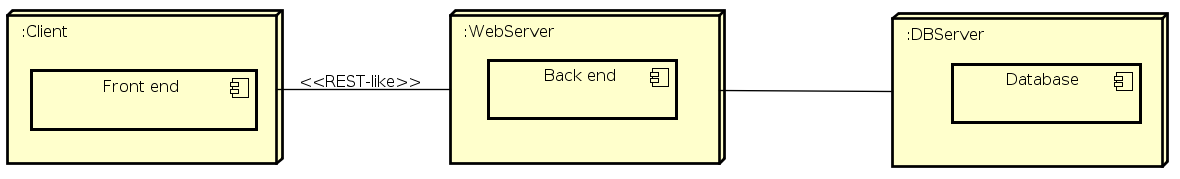
\includegraphics[width=0.8\textwidth]{res/sections/GeneralArchitecture.png}
\caption{Diagramma di deployment per l'architettura}
\end{figure}
\subsection{Interfaccia REST like}
Il back end si basa su uno stile REST like. Dal login al logout l'interfaccia di accesso ai dati può considerarsi a tutti gli effetti REST, ovvero con le seguenti caratteristiche:
\begin{itemize}
\item stato dell'applicazione e funzionalità divisi in risorse web;
\item ogni risorsa è unica e indirizzabile attraverso un URI (\textbf{U}niform \textbf{R}esource \textbf{I}dentifier);
\item tutte le risorse sono condivise come interfaccia uniforme per il trasferimento di stato tra client e risorse. Questo trasferimento consiste in:
\begin{itemize}
\item un insieme vincolato di operazioni ben definite;
\item un insieme vincolato di contenuti, opzionalmente supportato da codice a richiesta;
\item un protocollo:
\begin{itemize}
\item client-server;
\item privo di stato;
\item memorizzabile in cache;
\item a livelli.
\end{itemize}
\end{itemize}
\end{itemize}
REST utilizza il concetto di risorsa (aggregato di dati con un nome, l'URI, e una rappresentazione interna), sulla quale è possibile invocare operazioni CRUD (\textbf{C}reate, \textbf{R}ead, \textbf{U}pdate, \textbf{D}elete) con la seguente corrispondenza:
\begin{table}[H]
\centering
\label{CRUD}
\begin{tabular}{| >{\centering}p{3cm} | >{\centering}p{5cm} | >{\centering}p{6cm} |}
\hline
\textbf{Risorsa} & \textbf{URI della collection} \newline es. http://maas.com/users & \textbf{URI della risorsa} \newline es. http://maas.com/users/10 \tabularnewline \hline
\textbf{GET} & Fornisce informazioni sui membri della collection. & Fornisce una rappresentazione dell'elemento della collection indicato. \tabularnewline \hline
\textbf{PUT} & Non usata. & Sostituisce una rappresentazione dell'elemento della collection indicato. Se non esiste lo crea.  \tabularnewline \hline
\textbf{POST} & Crea un nuovo elemento della collection. La URI del nuovo elemento è generata automaticamente. & Non usato. \tabularnewline \hline
\textbf{DELETE} & Non usata. & Cancella l'elemento della collection indicato. \tabularnewline \hline
\end{tabular}
\caption{Tabella delle operazioni CRUD}
\end{table}
Per la rappresentazione dei dati si è scelto di utilizzare JSON (\textbf{J}ava\textbf{S}cript \textbf{O}bject \textbf{N}otation) perché si integra molto bene con i framework utilizzati e con il linguaggio JavaScript. Questo non è vero per XML (e\textbf{X}tensible \textbf{M}arkup \textbf{L}anguage) o CSV (\textbf{C}omma \textbf{S}eparated \textbf{V}alues), che richiederebbero librerie specifiche. Inoltre JSON è molto meno verboso e molto più flessibile di XML, e si adatta molto bene al dominio dell'applicazione.
\subsubsection{Backend}
%todo
\subsubsection{Frontend}
%todo